\section[M1: Metamodell]{M1: Meta-Modellierung}
\begin{frame}{Meta-Modellierung}
	\centering
	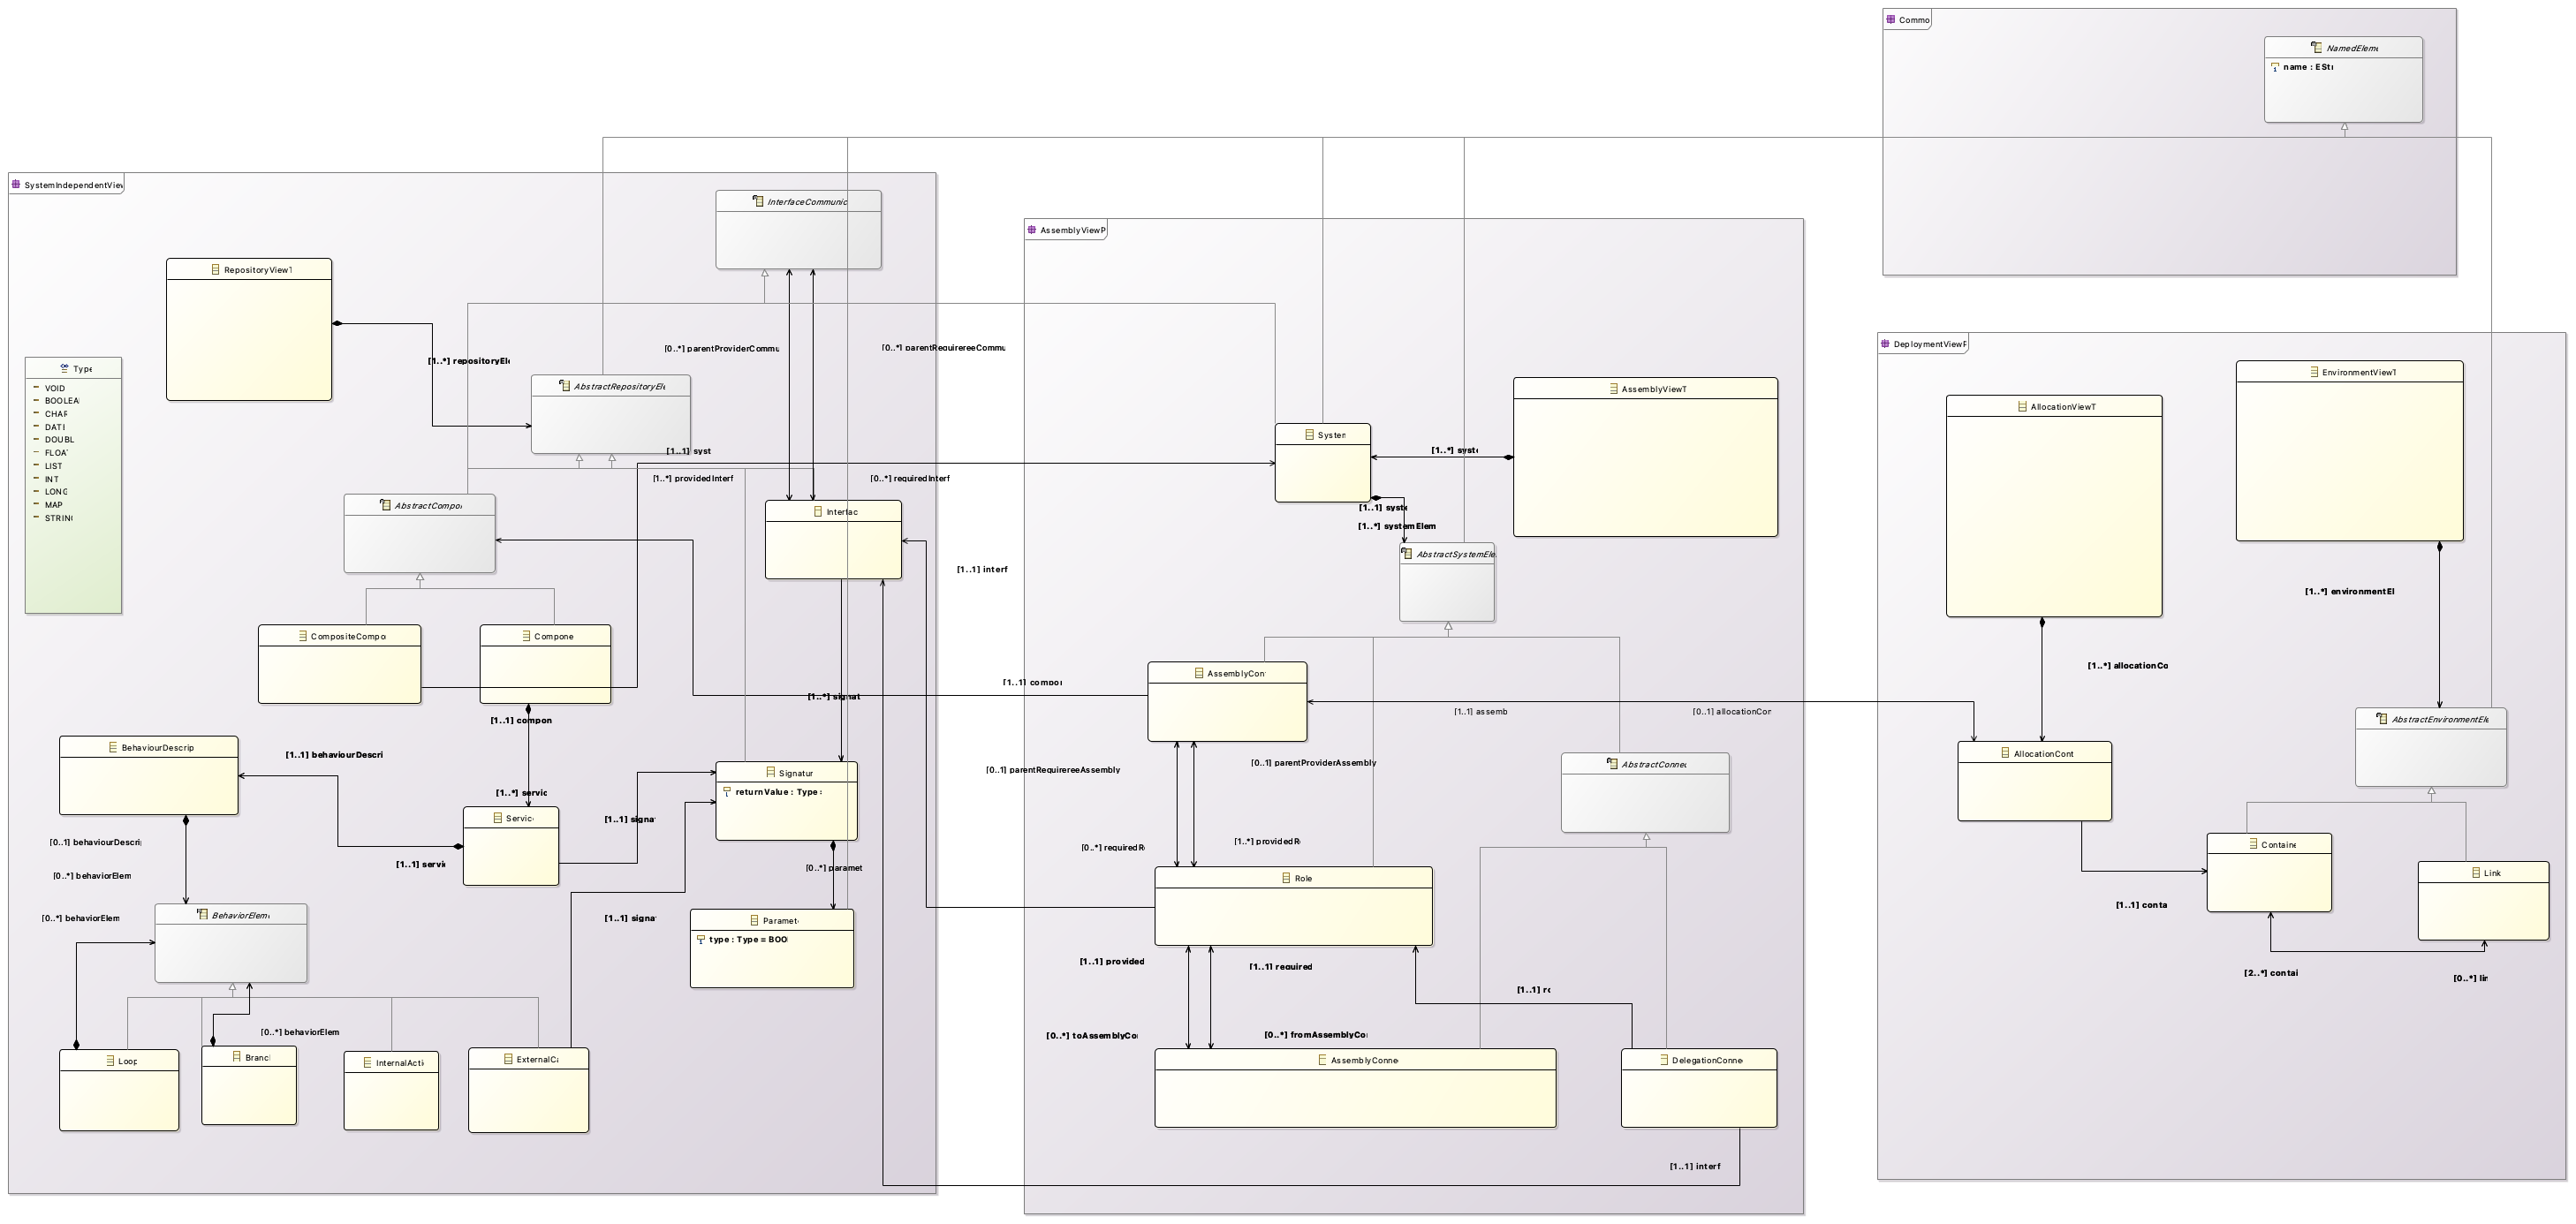
\includegraphics[height=60mm]{figures/meta-modell.png}
\end{frame}

\begin{frame}{Entwurfsentscheidungen für die Meta-Modellierung}
	\begin{enumerate}
		\item Verwendung von 4 Packages
		\begin{itemize}
			\item klare Trennung der View Points
			\item Nachteil für spätere Entwicklung
		\end{itemize}
		\item Common Package für wiederverwendbare Elemente
		\item ENUM zur Modellierung des \texttt{Type}
		\item Verwendung von OCL
		\item \item Designentscheidung: weniger oder mehr Informationen am Anfang beschreiben beeinflusst wie man mit dem Meta-Modell weiterarbeiten kann
	\end{enumerate}
\end{frame}